\documentclass[11pt,a4paper]{article}

% --- PACKAGES ---
\usepackage{fontspec}
\setmainfont{Times New Roman}
\setmonofont{Consolas}[Scale=0.92]

\usepackage[top=2.2cm, bottom=2.2cm, left=2.2cm, right=2.2cm]{geometry}
\setlength{\headheight}{24pt}
\addtolength{\topmargin}{-12pt}

\usepackage{xcolor}
\usepackage{amssymb}
\usepackage{tcolorbox}
\tcbuselibrary{skins}
\usepackage{tikz}
\usetikzlibrary{shapes.geometric, arrows.meta, positioning, calc, shadows}
\usepackage{booktabs}
\usepackage{tabularx}
\usepackage{multirow}
\usepackage{listings}
\usepackage{fancyhdr}
\usepackage{lastpage}
\usepackage{enumitem}
\usepackage{titlesec}
\usepackage{microtype}
\usepackage{caption}
\usepackage{hyperref}
\usepackage{xurl}

% --- COLOR DEFINITIONS ---
\definecolor{primaryblue}{HTML}{0F3460}
\definecolor{secondaryteal}{HTML}{0D9488}
\definecolor{accentgold}{HTML}{D97706}
\definecolor{darkgray}{HTML}{1F2937}
\definecolor{lightgray}{HTML}{F3F4F6}
\definecolor{boxbg}{HTML}{F8FAFC}
\definecolor{borderblue}{HTML}{93C5FD}
\definecolor{codegreen}{HTML}{15803D}
\definecolor{codegray}{HTML}{6B7280}
\definecolor{codepurple}{HTML}{7E22CE}
\definecolor{codebg}{HTML}{F8FAFC}

% --- HYPERREF SETUP ---
\hypersetup{
    colorlinks=true,
    linkcolor=primaryblue,
    citecolor=secondaryteal,
    urlcolor=secondaryteal,
    pdftitle={DSAI1003 - Course Handbook and Effective Python Self-Study Guide},
    pdfauthor={Dr. Vu Duc Minh - National Economics University (NEU)},
    pdfkeywords={Python, DSAI1003, Self-Study, AI Tutor, NEU, DSFE}
}

% --- HEADERS & FOOTERS ---
\pagestyle{fancy}
\fancyhf{}
\renewcommand{\headrulewidth}{0.6pt}
\renewcommand{\headrule}{\hbox to\headwidth{\color{primaryblue}\leaders\hrule height \headrulewidth\hfill}}
\fancyhead[L]{\small\color{primaryblue}\textbf{DSAI1003: Fundamental Programming Concepts in Python}}
\fancyhead[R]{\small\color{gray}Course Handbook \& Self-Study Guide}
\fancyfoot[L]{\small\color{gray}School of Technology -- National Economics University (NEU)}
\fancyfoot[R]{\small\color{primaryblue}\textbf{Page \thepage\ of \pageref{LastPage}}}

% --- SECTION FORMATTING ---
\titleformat{\section}
  {\Large\bfseries\color{primaryblue}}
  {\thesection.}{0.8em}{}
  [{\color{secondaryteal}\titlerule[1.5pt]}]

\titleformat{\subsection}
  {\large\bfseries\color{primaryblue}}
  {\thesubsection}{0.6em}{}

\titleformat{\subsubsection}
  {\normalsize\bfseries\color{secondaryteal}}
  {\thesubsubsection}{0.5em}{}

\titlespacing*{\section}{0pt}{14pt}{8pt}
\titlespacing*{\subsection}{0pt}{10pt}{5pt}
\titlespacing*{\subsubsection}{0pt}{8pt}{4pt}

% --- CUSTOM TCOLORBOX BOXES ---
\newtcolorbox{infobox}[1]{
    enhanced,
    colback=boxbg,
    colframe=primaryblue,
    arc=4pt,
    boxrule=1pt,
    leftrule=5pt,
    title=\textbf{#1},
    coltitle=white,
    colbacktitle=primaryblue,
    attach boxed title to top left={yshift=-2mm, xshift=4mm},
    boxed title style={arc=2pt, boxrule=0pt},
    fonttitle=\small\bfseries,
    top=4mm, bottom=3mm, left=3mm, right=3mm
}

\newtcolorbox{tipbox}[1]{
    enhanced,
    colback=boxbg,
    colframe=secondaryteal,
    arc=4pt,
    boxrule=1pt,
    leftrule=5pt,
    title=\textbf{#1},
    coltitle=white,
    colbacktitle=secondaryteal,
    attach boxed title to top left={yshift=-2mm, xshift=4mm},
    boxed title style={arc=2pt, boxrule=0pt},
    fonttitle=\small\bfseries,
    top=4mm, bottom=3mm, left=3mm, right=3mm
}

\newtcolorbox{warningbox}[1]{
    enhanced,
    colback=boxbg,
    colframe=accentgold,
    arc=4pt,
    boxrule=1pt,
    leftrule=5pt,
    title=\textbf{#1},
    coltitle=white,
    colbacktitle=accentgold,
    attach boxed title to top left={yshift=-2mm, xshift=4mm},
    boxed title style={arc=2pt, boxrule=0pt},
    fonttitle=\small\bfseries,
    top=4mm, bottom=3mm, left=3mm, right=3mm
}

\newtcolorbox{promptbox}[1]{
    enhanced,
    colback=lightgray!50,
    colframe=darkgray,
    arc=3pt,
    boxrule=0.8pt,
    leftrule=4pt,
    title=\textbf{Actionable Prompt Template: #1},
    coltitle=white,
    colbacktitle=darkgray,
    attach boxed title to top left={yshift=-2mm, xshift=4mm},
    boxed title style={arc=2pt, boxrule=0pt},
    fonttitle=\small\bfseries,
    top=4mm, bottom=3mm, left=3mm, right=3mm
}

% --- LISTINGS CONFIGURATION ---
\lstdefinestyle{mypython}{
    backgroundcolor=\color{codebg},
    commentstyle=\color{codegray}\itshape,
    keywordstyle=\color{primaryblue}\bfseries,
    numberstyle=\tiny\color{codegray},
    stringstyle=\color{codegreen},
    basicstyle=\small\ttfamily,
    breakatwhitespace=false,
    breaklines=true,
    captionpos=b,
    keepspaces=true,
    numbers=left,
    numbersep=7pt,
    showspaces=false,
    showstringspaces=false,
    showtabs=false,
    tabsize=4,
    frame=single,
    rulecolor=\color{borderblue},
    xleftmargin=12pt,
    framexleftmargin=8pt
}
\lstset{style=mypython}

% --- TIKZ STYLES ---
\tikzset{
    startstop/.style={rectangle, rounded corners=4pt, minimum width=3.2cm, minimum height=0.75cm, text centered, align=center, draw=primaryblue, fill=primaryblue!10, font=\small\bfseries},
    process/.style={rectangle, rounded corners=3pt, minimum width=3.2cm, minimum height=0.68cm, text centered, align=center, draw=secondaryteal, fill=secondaryteal!10, font=\small},
    arrow/.style={thick, ->, >=stealth, color=primaryblue}
}

\begin{document}

% ==================== HEADER BANNER / TITLE PAGE ====================
\begin{tcolorbox}[
    enhanced,
    colback=primaryblue,
    colframe=primaryblue,
    arc=5pt,
    boxrule=0pt,
    top=6mm, bottom=6mm, left=6mm, right=6mm
]
\begin{center}
    {\color{white}\large\textbf{NATIONAL ECONOMICS UNIVERSITY -- SCHOOL OF TECHNOLOGY}}\\[1mm]
    {\color{white}\small\textbf{FACULTY OF DATA SCIENCE AND ARTIFICIAL INTELLIGENCE}}\\[4mm]
    {\color{white}\Huge\textbf{COURSE HANDBOOK \& SELF-STUDY GUIDE}}\\[2mm]
    {\color{accentgold}\Large\textbf{DSAI1003: FUNDAMENTAL PROGRAMMING CONCEPTS IN PYTHON}}\\[1mm]
    {\color{white!80}\small\textit{Fundamental Programming Concepts in Python}}
\end{center}
\end{tcolorbox}

\vspace{2mm}

\begin{tcolorbox}[
    enhanced,
    colback=white,
    colframe=borderblue,
    arc=4pt,
    boxrule=1pt,
    top=3mm, bottom=3mm, left=4mm, right=4mm
]
\begin{tabularx}{\textwidth}{@{}lXlX@{}}
    \textbf{Instructor:} & Dr. Vu Duc Minh & \textbf{Program:} & Data Science in Finance \& E-commerce (DSFE) \\
    \textbf{Course Code:} & DSAI1003 & \textbf{Workload:} & 3 Credits (45h Lectures + 22.5h Lab + 90h Self-study) \\
    \textbf{Decision:} & 975/QĐ-ĐHKTQD (30/03/2024) & \textbf{Course Type:} & Compulsory Core Foundation \\
    & \textbf{Website:} & \href{https://vudmvn.github.io/Fundamental-of-Programming-Concepts-in-Python/}{vudmvn.github.io/Fundamental-of-Programming-Concepts-in-Python} \\
\end{tabularx}
\end{tcolorbox}

\vspace{3mm}

% ==================== TABLE OF CONTENTS ====================
\tableofcontents

\vspace{5mm}

% ==================== SECTION 1 ====================
\section{Course Overview \& Detailed Syllabus}

\subsection{Course Description \& Pedagogical Philosophy}
The course \textbf{Fundamental Programming Concepts in Python (DSAI1003)} is an introductory prerequisite course in the Bachelor of Data Science in Finance and E-commerce (DSFE) program. It is designed to establish a solid foundation in algorithmic thinking, program structure, and computational problem-solving using Python.

\begin{infobox}{Key Characteristics of the Course Approach}
\begin{itemize}[leftmargin=1.5em, itemsep=2pt]
    \item \textbf{No prior programming experience required:} Students only need a solid grasp of high school algebra and fundamental logical thinking skills.
    \item \textbf{Practical real-world orientation:} Examples, coding exercises, and case studies are drawn directly from economics, corporate finance, retail transactions, and e-commerce.
    \item \textbf{Systematic pedagogical progression:} Students start from algorithmic design (pseudocode, flowcharts), master fundamental control structures, implement modular functions, leverage versatile built-in collections, and culminate in Object-Oriented Programming (OOP) fundamentals.
\end{itemize}
\end{infobox}

\subsection{Course Objectives (COs) \& Learning Outcomes (CLOs)}
The course aims to fulfill 7 overarching objectives (\textbf{G1} through \textbf{G7}), mapped to measurable Program Learning Outcomes (PLOs):

\begin{table}[htbp]
\centering
\small
\begin{tabularx}{\textwidth}{@{}c X c c@{}}
\toprule
\textbf{No.} & \textbf{Course Objective Description (COs)} & \textbf{PLO} & \textbf{Level} \\
\midrule
\textbf{G1} & Implement simple console programs or graphical user-interface programs to solve business problems. & 1.4, 2.2 & 4 \\
\textbf{G2} & Use decision structures (\texttt{if-elif-else}) and loop structures (\texttt{while}, \texttt{for}) for repetitive tasks. & 1.4, 2.2 & 4 \\
\textbf{G3} & Design and implement modular functions and recursive functions for divide-and-conquer tasks. & 1.4, 2.2 & 4 \\
\textbf{G4} & Proficiently utilize built-in data collections (\texttt{List}, \texttt{Tuple}, \texttt{Set}, \texttt{Dictionary}) to process data. & 1.4, 2.2 & 4 \\
\textbf{G5} & Implement file I/O operations (text, binary) and handle exceptions safely (\texttt{try-except}). & 1.4, 2.2 & 4 \\
\textbf{G6} & Acquire and apply core Object-Oriented Programming (OOP: Classes, Inheritance, Polymorphism). & 1.4, 2.2 & 3 \\
\textbf{G7} & Develop self-study ability, independent problem-solving, teamwork, and personal accountability. & 2.4, 3.1 & 3 \\
\bottomrule
\end{tabularx}
\caption{DSAI1003 Course Objectives Mapping}
\end{table}

\subsection{Textbooks \& Learning Resources}
The curriculum integrates three internationally recognized textbooks:
\begin{enumerate}[leftmargin=1.5em, itemsep=3pt]
    \item \textbf{[1] Python for Everyone} (3rd Edition, 2019) -- \textit{Cay Horstmann, Rance Necaise}, John Wiley \& Sons. (Main textbook for syntax, algorithmic patterns, and business applications).
    \item \textbf{[2] Intro to Python for Computer Science and Data Science: Learning to Program with AI, Big Data and The Cloud} (2020) -- \textit{Paul Deitel, Harvey Deitel}, Pearson Education. (Main textbook for data processing mindset and modern AI applications).
    \item \textbf{[3] The Python Workbook: A Brief Introduction with Exercises and Solutions} (2nd Edition, 2019) -- \textit{Ben Stephenson}, Springer. (Self-study exercises with comprehensive solutions).
\end{enumerate}

\subsection{Assessment Scheme \& Course Regulations}
Academic performance is assessed through 3 independent components, ensuring continuous feedback and accurate measurement of practical programming competence:

\begin{table}[htbp]
\centering
\small
\begin{tabularx}{\textwidth}{@{}l X c p{4.2cm} c@{}}
\toprule
\textbf{Assessment Component} & \textbf{Scope \& Content} & \textbf{Timing} & \textbf{Criteria \& Tools} & \textbf{Weight} \\
\midrule
\textbf{Homework (HW)} & Theoretical questions \& coding assignments & Bi-weekly ($\ge$ 4 sets) & Algorithmic logic, code clarity, deadline compliance (LMS) & \textbf{30\%} \\
\textbf{Midterm Exam} & Core concepts \& algorithms (Lessons 1--6) & Week 7 & Written test or lab computer exam & \textbf{30\%} \\
\textbf{Final Exam} & Comprehensive practical programming (Lessons 1--10) & Week 15 & Lab computer practical test (execution, OOP, error handling) & \textbf{40\%} \\
\bottomrule
\end{tabularx}
\caption{DSAI1003 Course Assessment Scheme}
\end{table}

\begin{warningbox}{Important Course Regulations}
\begin{itemize}[leftmargin=1.5em, itemsep=2pt]
    \item \textbf{Attendance:} Students are required to attend a minimum of \textbf{80\%} of scheduled class sessions.
    \item \textbf{Passing requirement:} The final weighted course grade must be at least \textbf{5.0 / 10.0}.
    \item \textbf{Classroom laptops:} Personal laptops may only be used during designated hands-on coding exercises under instructor guidance; unauthorized non-academic activities are strictly prohibited.
\end{itemize}
\end{warningbox}

\subsection{15-Week Detailed Course Schedule}
The 15-week semester is organized into 2 distinct pedagogical phases:

\subsubsection*{Phase 1: Syntax Foundations, Control Structures \& Algorithms (Weeks 1 -- 7)}
\begin{table}[htbp]
\centering
\footnotesize
\begin{tabularx}{\textwidth}{@{}c p{5.5cm} p{2.8cm} X@{}}
\toprule
\textbf{Week} & \textbf{Topic \& Core Content} & \textbf{Reading} & \textbf{Activities \& Assessment} \\
\midrule
\textbf{1} & \textbf{Lesson 1: Introduction \& Algorithms}\newline Computer architectures, Python interpreter, compilation vs. runtime errors, pseudocode, flowcharts. & [1] Ch. 1\newline [2] Ch. 1 & Syllabus introduction, environment setup (Python 3.11+, VS Code, Google Colab). \\
\midrule
\textbf{2} & \textbf{Lesson 2: Software Process \& Data Types}\newline Numbers, strings, arithmetic expressions, assignments, variables, built-in functions. & [1] Ch. 2\newline [2] Ch. 2, 4 & Live coding, interactive Q\&A. Assign \textbf{Homework \#1}. \\
\midrule
\textbf{3} & \textbf{Lesson 3: Decision Structures}\newline Statements \texttt{if}, \texttt{if-else}, \texttt{if-elif-else}, Boolean logic and truth tables. & [1] Ch. 3\newline [2] Ch. 3 & Branching practice, branch coverage testing. Due: Homework \#1. \\
\midrule
\textbf{4} & \textbf{Lesson 4: Loop Structures}\newline Loops \texttt{while}, \texttt{for}, nested iterations, string indexing and traversals. & [1] Ch. 4\newline [2] Ch. 3 & Accumulator and sentinel loop patterns. Assign \textbf{Homework \#2}. \\
\midrule
\textbf{5} & \textbf{Lesson 5: Function Design}\newline Syntax \texttt{def}, parameters, return values, variable scope, recursion basics. & [1] Ch. 5\newline [2] Ch. 4 & Modularization and divide-and-conquer. Due: Homework \#2. \\
\midrule
\textbf{6} & \textbf{Lesson 6: Lists \& Tuples}\newline Linear arrays, negative indexing, slicing, List methods, 2D nested tables. & [1] Ch. 6\newline [2] Ch. 5 & Tabular data structures and operations. Assign \textbf{Homework \#3}. \\
\midrule
\textbf{7} & \textbf{Midterm Exam}\newline Comprehensive review \& evaluation of Lessons 1 through 6. & [1] Lessons 1--6 & \textbf{Midterm Examination (Weight: 30\%)}. \\
\bottomrule
\end{tabularx}
\caption{Course Schedule: Phase 1 (Weeks 1 -- 7)}
\end{table}

\subsubsection*{Phase 2: Advanced Collections, File I/O \& Object-Oriented Programming (Weeks 8 -- 15)}
\begin{table}[htbp]
\centering
\footnotesize
\begin{tabularx}{\textwidth}{@{}c p{5.5cm} p{2.8cm} X@{}}
\toprule
\textbf{Week} & \textbf{Topic \& Core Content} & \textbf{Reading} & \textbf{Activities \& Assessment} \\
\midrule
\textbf{8--9} & \textbf{Lesson 7: File I/O \& Exception Handling}\newline Text file reading/writing, \texttt{sys.argv}, defensive error handling (\texttt{try-except}). & [1] Ch. 7\newline [2] Ch. 4 & Persistent data storage \& robust software design. Assign \textbf{Homework \#4}. \\
\midrule
\textbf{10} & \textbf{Lesson 8: Sets \& Dictionaries}\newline Hash tables, key-value mappings, set operations, nested JSON-like records. & [1] Ch. 8\newline [2] Ch. 6 & Commercial transaction data processing \& business analytics. \\
\midrule
\textbf{11--12} & \textbf{Lesson 9: Objects \& Classes (OOP -- Part 1)}\newline OOP philosophy, \texttt{class} declarations, \texttt{\_\_init\_\_} constructor, encapsulation, instance methods. & [1] Ch. 9\newline [2] Ch. 10 & Modeling banking and invoice entities. In-class OOP mini-lab. \\
\midrule
\textbf{13--14} & \textbf{Lesson 10: Inheritance \& Polymorphism (OOP -- Part 2)}\newline Inheritance hierarchy, subclassing, \texttt{super()}, method overriding, polymorphism. & [1] Ch. 10\newline [2] Ch. 10 & Advanced OOP software architecture. Final exam review guidelines. \\
\midrule
\textbf{15} & \textbf{Course Review \& Final Exam Prep}\newline Comprehensive synthesis of DSAI1003, instructor Q\&A session. & All resources & Computer lab mock test \& hands-on skills consolidation. \\
\bottomrule
\end{tabularx}
\caption{Course Schedule: Phase 2 (Weeks 8 -- 15)}
\end{table}

% ==================== SECTION 2 ====================
\newpage
\section{Effective Python Self-Study Methodology}

\subsection{The Nature of Learning Programming \& 4 Fatal Pitfalls}
Learning programming differs fundamentally from memorizing theoretical subjects or rote syntax memorization. \textbf{The essence of programming is systematic problem-solving: decomposing problems and translating algorithms into precise computer instructions.}

\begin{tipbox}{Core Self-Study Principle}
\textit{"Learn programming by reading less, practicing more, and thinking before looking at solutions."}
\end{tipbox}

Novice programmers frequently stumble into four psychological pitfalls:
\begin{enumerate}[leftmargin=1.5em, itemsep=3pt]
    \item \textbf{The Illusion of Competence via Passive Reading (Reading without running):} Skimming sample code and thinking \textit{"I understand this"}. When the screen is turned off, the learner cannot write a single line from scratch.
    \item \textbf{Blind Copy-Pasting:} Code executes, but the learner cannot explain why specific statements exist or what the parameters signify.
    \item \textbf{Checking Solutions Prematurely:} Giving up and opening the answer immediately upon encountering difficulty. This bypasses the critical mental struggle where genuine problem-solving capacity is built.
    \item \textbf{Cramming Too Many Concepts Simultaneously:} Attempting to rush through Variables $\rightarrow$ Branching $\rightarrow$ Loops $\rightarrow$ Functions $\rightarrow$ OOP in two days without allowing time for concepts to consolidate through deliberate practice.
\end{enumerate}

\subsection{The 9-Step Active Study Cycle}
To truly master a programming concept, students are strongly advised to follow this closed-loop learning cycle:

\begin{figure}[htbp]
\centering
\begin{tikzpicture}[node distance=1.05cm]
    \node (step1) [startstop] {1. Read};
    \node (step2) [process, below of=step1] {2. Explain (Own Words)};
    \node (step3) [process, below of=step2] {3. Predict Output};
    \node (step4) [process, below of=step3] {4. Run Code};
    \node (step5) [process, below of=step4] {5. Modify \& Experiment};
    \node (step6) [process, below of=step5] {6. Practice Independently};
    \node (step7) [process, below of=step6] {7. Debug \& Fix Errors};
    \node (step8) [process, below of=step7] {8. Review Performance};
    \node (step9) [startstop, below of=step8] {9. Reflect \& Log};

    \draw [arrow] (step1) -- (step2);
    \draw [arrow] (step2) -- (step3);
    \draw [arrow] (step3) -- (step4);
    \draw [arrow] (step4) -- (step5);
    \draw [arrow] (step5) -- (step6);
    \draw [arrow] (step6) -- (step7);
    \draw [arrow] (step7) -- (step8);
    \draw [arrow] (step8) -- (step9);
    \draw [arrow] (step9.east) -- ++(1.4,0) -- ++(0,8.4) -- (step1.east);
\end{tikzpicture}
\caption{The 9-Step Active Programming Study Cycle}
\end{figure}

Self-study time should not be distributed equally across steps. \textbf{Over 70\% of study time must be spent directly on: typing code, observing runtime behavior, analyzing tracebacks, and solving unassisted exercises (The 70/30 Rule).}

\subsection{Breakthrough Active Learning Techniques}

\subsubsection{The Predict \texorpdfstring{$\rightarrow$}{->} Run \texorpdfstring{$\rightarrow$}{->} Explain Technique}
Before clicking the Run button on your IDE, force yourself to write down on paper or predict mentally:
\begin{itemize}[leftmargin=1.5em, itemsep=2pt]
    \item Exactly what text or numbers will appear on the screen?
    \item How does each line change variable states and memory contents?
\end{itemize}
When actual execution differs from your prediction, that discrepancy marks the exact moment your mental model of Python's execution model is upgraded.

\subsubsection{The Teach-Back Technique}
Explain a concept (e.g., \textit{"How does a function return value differ from a print statement?"}) to someone without a technical background, or record your explanation. If you find yourself saying: \textit{"It runs like that because that is how it is"}, you have not yet mastered the underlying mechanism.

\subsubsection{Active Recall \& Spaced Repetition}
Avoid rereading slides repeatedly. Close all materials and answer diagnostic questions: \textit{What data type does \texttt{input()} return? How do you cast to an integer? What error occurs if you concatenate a string with an integer?} Schedule reviews after 1 day, 3 days, 7 days, and 14 days to transform transient memory into enduring intuition.

\subsection{The 5-Level Learning Ladder}
Whenever tackling a new programming topic, ascend systematically through these difficulty tiers:
\begin{itemize}[leftmargin=1.5em, itemsep=3pt]
    \item \textbf{Level 1 -- Modify Existing Code:} Change variable values, convert integers to floats, observe corresponding output changes.
    \item \textbf{Level 2 -- Reconstruct from Description:} Cover the solution, read the problem prompt, and write the complete program from scratch.
    \item \textbf{Level 3 -- Combine Multiple Concepts:} For instance: Combine a \texttt{for} loop with an \texttt{if-else} branch to filter even and odd integers from a list.
    \item \textbf{Level 4 -- Real-World Contextual Problems:} Compute progressive electricity tariffs, calculate personal income tax brackets, or model compound interest.
    \item \textbf{Level 5 -- Mini Project:} Build a console-based order management system or an expense transaction analyzer.
\end{itemize}

\subsection{Standard Debugging Checklist \& Error Categories}
Encountering errors is inevitable and an essential component of learning programming. When your program crashes, do not panic or randomly delete code. Apply this structured checklist:

\begin{infobox}{Standard 8-Step Debugging Protocol}
\begin{enumerate}[leftmargin=1.5em, itemsep=2pt]
    \item Read the entire traceback message from the bottom line upward.
    \item Pinpoint the exact file and line number where the failure occurred.
    \item Identify the specific error class: \textbf{SyntaxError}, \textbf{NameError}, \textbf{TypeError}, \textbf{IndexError}, \textbf{ZeroDivisionError}.
    \item Insert temporary \texttt{print()} statements or use a debugger to inspect real-time variable values.
    \item Verify variable types using \texttt{type()}.
    \item Compare observed runtime output with theoretical expectations.
    \item Test the program against the smallest, simplest possible input data.
    \item Change only \textbf{one variable or line at a time} between test executions.
\end{enumerate}
\end{infobox}

\subsection{Building a Personal Learning Log \& Error Log}
Dedicate 5 minutes after every study session to update your personal log (\texttt{learning\_log.md}):

\begin{table}[htbp]
\centering
\small
\begin{tabularx}{\textwidth}{@{}p{4.2cm} X p{3.6cm} c@{}}
\toprule
\textbf{Encountered Error} & \textbf{Root Cause} & \textbf{Resolution Strategy} & \textbf{Understood?} \\
\midrule
\texttt{TypeError: can only concatenate str to str} & \texttt{input()} always returns a string (\texttt{str}), which cannot be directly added to integers. & Cast with \texttt{int(input())} or \texttt{float(input())} before math operations. & Yes \\
\midrule
\texttt{IndexError: list index out of range} & Iteration reached index $N$, while the valid list indices range from $0$ to $N-1$. & Adjust boundaries using \texttt{range(len(lst))}. & Yes \\
\midrule
Infinite while loop & Failed to increment the loop counter inside the \texttt{while} body. & Append \texttt{i += 1} at the end of the loop body. & Yes \\
\bottomrule
\end{tabularx}
\caption{Sample Personal Error Log}
\end{table}

% ==================== SECTION 3 ====================
\newpage
\section{Strategic Use of Artificial Intelligence (AI) in Learning}

\subsection{Accurate Positioning of AI in Programming Education}
Large Language Models (ChatGPT, Claude, Gemini) provide unprecedented educational leverage. However, their true pedagogical value depends entirely on \textbf{how learners interact with them}.

\begin{warningbox}{Hazards of AI Over-Reliance}
If a student merely pastes problem statements: \textit{"Solve this problem for me"} and copies the generated code:
\begin{itemize}[leftmargin=1.5em, itemsep=2pt]
    \item The student never grasps algorithmic construction or architectural design rationales.
    \item In proctored exams without AI access, the student is left entirely paralyzed.
    \item Over time, analytical reasoning and critical problem-solving capabilities suffer severe cognitive atrophy.
\end{itemize}
\end{warningbox}

\begin{tipbox}{Positioning AI: Personal Tutor \& Coach}
Treat AI as a dedicated \textbf{Personal Tutor and Coach}:
\begin{itemize}[leftmargin=1.5em, itemsep=2pt]
    \item Ask AI to \textbf{explain} difficult concepts using relatable analogies.
    \item Request \textbf{incremental hints} when stuck, rather than full solutions.
    \item Ask AI to \textbf{generate diagnostic quizzes} to assess your conceptual grasp.
    \item Submit your own hand-written code for \textbf{code review and optimization suggestions}.
\end{itemize}
\end{tipbox}

\subsection{The 4-Part Structured Prompt Framework}
To guide AI toward educational coaching rather than simply giving away answers, an effective prompt must embody four key components:

\begin{tcolorbox}[enhanced, colback=white, colframe=primaryblue, arc=3pt, boxrule=1pt]
\begin{tabularx}{\textwidth}{@{}l p{3.2cm} X@{}}
    \textbf{1. Context} & Who are you, what level are you at? & \textit{"I am a first-year student beginning foundational Python programming..."} \\
    \textbf{2. Problem} & Where precisely are you stuck? & \textit{"I struggle to differentiate between variable assignment and equality comparison..."} \\
    \textbf{3. Task} & What specific assistance do you need? & \textit{"Explain this with an everyday analogy and a short code snippet under 8 lines..."} \\
    \textbf{4. Constraint} & What boundaries must AI respect? & \textit{"Do not use advanced features like functions or classes; ask me 2 check questions without providing answers yet."} \\
\end{tabularx}
\end{tcolorbox}

\subsection{The 5T Interaction Principle}
A rigorous workflow between student and AI is captured by the \textbf{5T Principle}:

\begin{figure}[htbp]
\centering

\begin{tikzpicture}[
    every node/.style={align=center, font=\small},
    stepbox/.style={rectangle, rounded corners=4pt, draw=primaryblue, fill=primaryblue!8, minimum width=2.8cm, minimum height=1.1cm, text width=2.6cm, inner sep=3pt}
]
    \node[stepbox] (t1) at (0,0) {\textbf{\color{primaryblue}1. Think}\\[1mm]\scriptsize Independent Analysis};
    \node[stepbox] (t2) at (3.35,0) {\textbf{\color{primaryblue}2. Try}\\[1mm]\scriptsize Write Initial Code};
    \node[stepbox] (t3) at (6.7,0) {\textbf{\color{primaryblue}3. Talk}\\[1mm]\scriptsize Ask Targeted Questions};
    \node[stepbox] (t4) at (10.05,0) {\textbf{\color{primaryblue}4. Test}\\[1mm]\scriptsize Verify on Machine};
    \node[stepbox] (t5) at (13.4,0) {\textbf{\color{primaryblue}5. Teach-back}\\[1mm]\scriptsize Synthesize in Words};

    \draw[thick, ->, >=stealth, color=secondaryteal] (t1) -- (t2);
    \draw[thick, ->, >=stealth, color=secondaryteal] (t2) -- (t3);
    \draw[thick, ->, >=stealth, color=secondaryteal] (t3) -- (t4);
    \draw[thick, ->, >=stealth, color=secondaryteal] (t4) -- (t5);
\end{tikzpicture}
\caption{The 5T Principle for Effective AI Interaction}
\end{figure}

\begin{enumerate}[leftmargin=1.5em, itemsep=3pt]
    \item \textbf{Think:} Identify Inputs, Outputs, and algorithmic strategies before opening an AI chat.
    \item \textbf{Try:} Type an initial draft independently, even if incomplete or buggy.
    \item \textbf{Talk:} Query AI specifically on the pinpointed bottleneck; share existing code, observed errors, and expectations.
    \item \textbf{Test:} Never accept AI code on faith. Copy it into your IDE, run it, and stress-test it against edge cases.
    \item \textbf{Teach-back:} Close the chat window, articulate the mechanism in your own words, and record the lesson in your notebook.
\end{enumerate}

\subsection{The Three-Level Hint System}
When confronting challenging assignments, train your AI assistant to dispense guidance in three calibrated tiers:

\begin{infobox}{The 3-Level Scaffolding Framework}
\begin{itemize}[leftmargin=1.5em, itemsep=3pt]
    \item \textbf{Level 1: Idea Hint:} AI outlines the mathematical logic or algorithmic pattern without providing any code.
    \item \textbf{Level 2: Structure Hint:} AI indicates appropriate programming constructs (e.g., recommend a \texttt{for} loop nested with an \texttt{if} condition using the modulo operator \texttt{\%}).
    \item \textbf{Level 3: Scaffold Hint:} AI provides a skeletal code template with blank placeholders (\texttt{\# TODO}) so the student must implement the critical logic.
\end{itemize}
\end{infobox}

\subsection{Actionable Prompt Toolkit}
The following high-leverage prompts can be customized and utilized directly during self-study:

\begin{promptbox}{Explaining a New Concept (Concept Prompt)}
\small
I am a beginner learning Python. Please explain the concept of [CONCEPT NAME, e.g., Recursive Functions].\newline
Requirements:\newline
1. Explain the underlying intuition using simple language and an everyday analogy.\newline
2. Provide a clean, annotated Python code example under 10 lines.\newline
3. Point out 1 common pitfall or misconception that beginners frequently make.\newline
4. Formulate 2 short diagnostic questions to test my understanding; do not provide answers yet.
\end{promptbox}

\begin{promptbox}{Requesting Problem Hints (Socratic Hint)}
\small
I am working independently on this exercise: "[EXERCISE DESCRIPTION]"\newline
My current idea and code attempt:\newline
\texttt{[PASTE YOUR CODE ATTEMPT HERE]}\newline
I am currently blocked at step: [DESCRIBE BOTTLENECK].\newline
Requirement: DO NOT write the complete solution. Provide a LEVEL 1 HINT (conceptual or algorithmic suggestion) so I can continue thinking and coding on my own.
\end{promptbox}

\begin{promptbox}{Debugging Assistance (Root Cause Discovery)}
\small
I wrote the following Python code to achieve: [DESCRIBE INTENDED BEHAVIOR].\newline
My current code:\newline
\texttt{[PASTE CURRENT CODE HERE]}\newline
When executed, I encounter this error/unexpected output: [PASTE TRACEBACK OR OUTPUT].\newline
Requirements:\newline
1. Explain the root cause of this error.\newline
2. Identify the specific lines that require attention.\newline
3. Ask me a guiding question so I can correct the bug myself; DO NOT rewrite the code for me.
\end{promptbox}

\begin{promptbox}{Code Review and Optimization (Pythonic Style)}
\small
I have completed this programming problem and the code runs correctly:\newline
\texttt{[PASTE COMPLETE WORKING CODE HERE]}\newline
Please act as an experienced Python Instructor and Software Engineer:\newline
1. Evaluate code quality: variable naming conventions, readability, and structural modularity.\newline
2. Does this implementation handle potential edge cases safely?\newline
3. Suggest 1 concrete optimization to make the code more concise and idiomatic (Pythonic), explaining the rationale.
\end{promptbox}

\begin{promptbox}{Self-Quiz Generation}
\small
I have just completed studying these topics: [LIST TOPICS, e.g., Lists, Tuples, and Slicing].\newline
Please generate a 6-question diagnostic quiz for me:\newline
- 2 Multiple-Choice questions (4 options A, B, C, D; exactly 1 correct answer).\newline
- 2 Predict-the-Output questions (short code snippets under 5 lines).\newline
- 2 Find-the-Bug questions (short snippets containing exactly 1 bug to fix).\newline
Constraint: Keep questions within beginner scope. DO NOT show answers yet; wait for my responses before grading and providing explanations.
\end{promptbox}

\subsection{7-Point AI Verification Checklist}
Before accepting any AI-generated code or explanation, students must cross-examine it against this 7-point checklist:
\begin{itemize}[leftmargin=1.5em, itemsep=2pt]
    \item[$\square$] \textbf{1. Curriculum Compatibility:} Does the code avoid unintroduced external libraries or advanced concepts beyond the current lesson?
    \item[$\square$] \textbf{2. Practical Execution:} Have you copied the code into your IDE and verified clean execution without warnings or errors?
    \item[$\square$] \textbf{3. Exact Specification Match:} Does the terminal output match assignment requirements down to formatting and casing?
    \item[$\square$] \textbf{4. Boundary Testing:} Does the program function properly with inputs like 0, negative values, empty strings, or empty lists?
    \item[$\square$] \textbf{5. Standard Terminology:} Is the terminology consistent with the course's official textbook (\textit{Python for Everyone})?
    \item[$\square$] \textbf{6. Line-by-Line Explanation:} Can you point to every single line and explain precisely why it is there?
    \item[$\square$] \textbf{7. Independent Reproduction:} If the AI chat was deleted, could you rewrite the program independently within 10 minutes?
\end{itemize}

\vspace{3mm}

\begin{warningbox}{The Inviolable Golden Rule}
\centering
\Large\textbf{``NEVER SUBMIT OR PRESERVE SOURCE CODE\\[2mm]THAT YOU CANNOT THOROUGHLY EXPLAIN YOURSELF.''}
\end{warningbox}

% ==================== SECTION 4 ====================
\vspace{4mm}
\section{Week 1 Action Plan for Success}

To attain top academic honors (Grade A/A+) in \textbf{DSAI1003}, students should execute these concrete action items during the first week:

\begin{enumerate}[leftmargin=1.5em, itemsep=4pt]
    \item \textbf{Set up your computing environment:}
    \begin{itemize}
        \item Install the latest stable Python version (Python 3.11+) from \url{https://www.python.org/}.
        \item Install \textbf{Visual Studio Code (VS Code)} with the official \textit{Python Extension Pack}.
        \item Sign in to \textbf{Google Colab} to enable seamless interactive programming from any browser.
    \end{itemize}
    \item \textbf{Access and organize learning resources:}
    \begin{itemize}
        \item Bookmark the official course GitHub repository: \url{https://github.com/vudmvn/Fundamental-of-Programming-Concepts-in-Python}.
        \item Read the detailed syllabus (\texttt{syllabus-en.md}) and Chapter 1 of \textit{Python for Everyone}.
    \end{itemize}
    \item \textbf{Establish your personal self-study system:}
    \begin{itemize}
        \item Create a dedicated study directory named \texttt{DSAI1003\_Python/} on your laptop or Google Drive.
        \item Create a \texttt{learning\_log.md} file to document lessons, errors, and key insights weekly.
        \item Save the Prompt Toolkit into your notes app to facilitate thoughtful, disciplined AI interactions.
    \end{itemize}
\end{enumerate}

\vspace{5mm}

\begin{tcolorbox}[enhanced, colback=primaryblue!5, colframe=primaryblue, arc=4pt, boxrule=1pt, top=4mm, bottom=4mm, left=5mm, right=5mm]
\begin{center}
    {\large\bfseries\color{primaryblue}WISHING ALL DSFE STUDENTS}\\[2mm]
    {\bfseries\color{secondaryteal}AN INSPIRING SEMESTER, MASTERING COMPUTATIONAL THINKING}\\
    {\bfseries\color{secondaryteal}\& HARNESSING MODERN AI TO ELEVATE YOUR PROFESSIONAL POTENTIAL!}\\[4mm]
    \small
    \textbf{Faculty of Data Science and Artificial Intelligence -- School of Technology}\\
    \textbf{National Economics University (NEU)}\\
    \textit{Hanoi, Academic Year 2024 -- 2025}
\end{center}
\end{tcolorbox}

\end{document}